% =====================================================================
% Expt Fig 3: Compare ensembling to model-size scaling at matched compute.
% =====================================================================

% --- 3a: 4x4 grid overview ---

\begin{figure}[t]
\centering
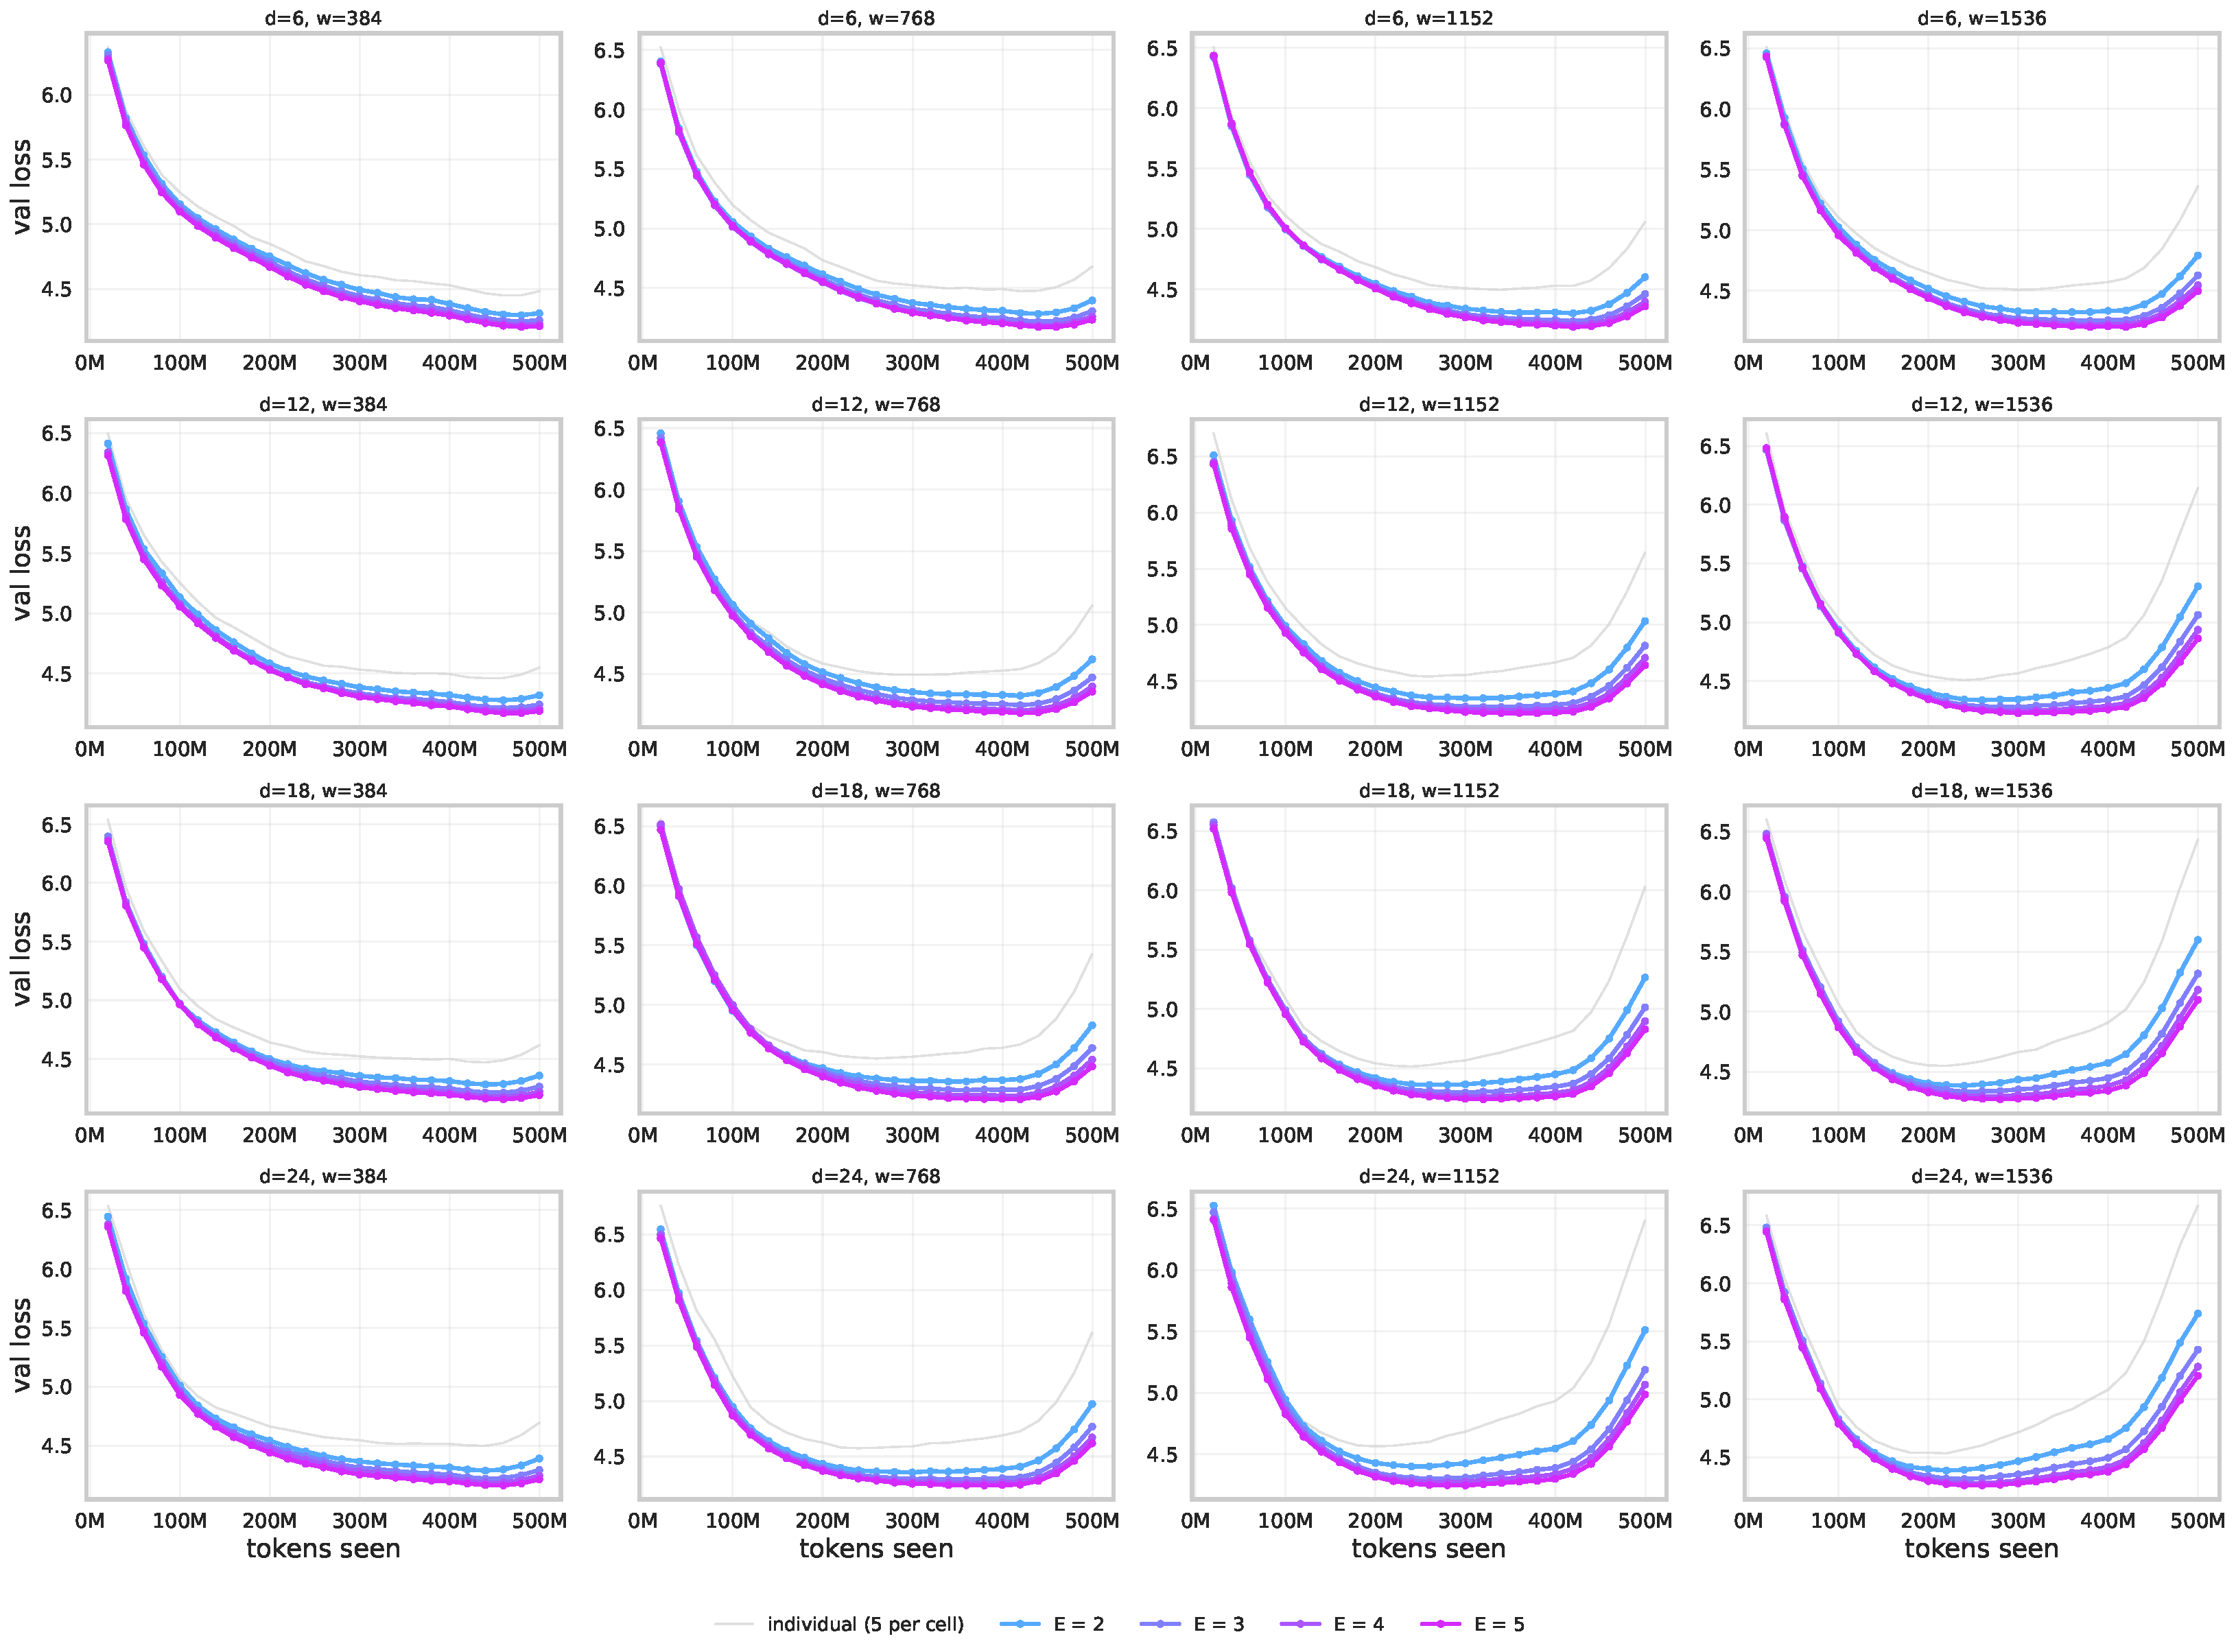
\includegraphics[width=0.99\linewidth]{experiments/figures/03_compute_matched/grid_4x4.pdf}
\caption{Validation loss versus cumulative tokens for all 16 cells of the $4 \times 4$ depth $\times$ width grid at $df=0.2$. Per cell: 5 individuals (gray) and ensemble val curves at $E \in \{2, 3, 4, 5\}$ (cool palette).}
\label{fig:grid_4x4}
\end{figure}

\paragraph{Notes on Figure~\ref{fig:grid_4x4}.}
Rows index depth $L \in \{6, 12, 18, 24\}$, columns index width $N \in \{384, 768, 1152, 1536\}$.
The full-set $4 \times 4$ grid combines the original 9-cell sweep ($L \in \{6, 12, 24\}$ $\times$ $N \in \{384, 768, 1536\}$) with the interpolated extension that adds the $L = 18$ row and the $N = 1152$ column.
All cells use the same setup: 25 epochs at $df=0.2$ on a 100M-token FineWeb subset, trapezoidal LR with linear warmdown, weight decay $0.1$, CompleteP, no value-embedding projections.
Strategy shown is init plus shuffle (per-epoch independent permutations); the init-only strategy is qualitatively similar.
The U-curve shape becomes more pronounced toward the bottom-right (deeper plus wider models), where overfit-onset is earlier in tokens and the post-onset climb is steeper.


% --- 3b/c: compute-matched comparison ---

\begin{figure}[t]
\centering
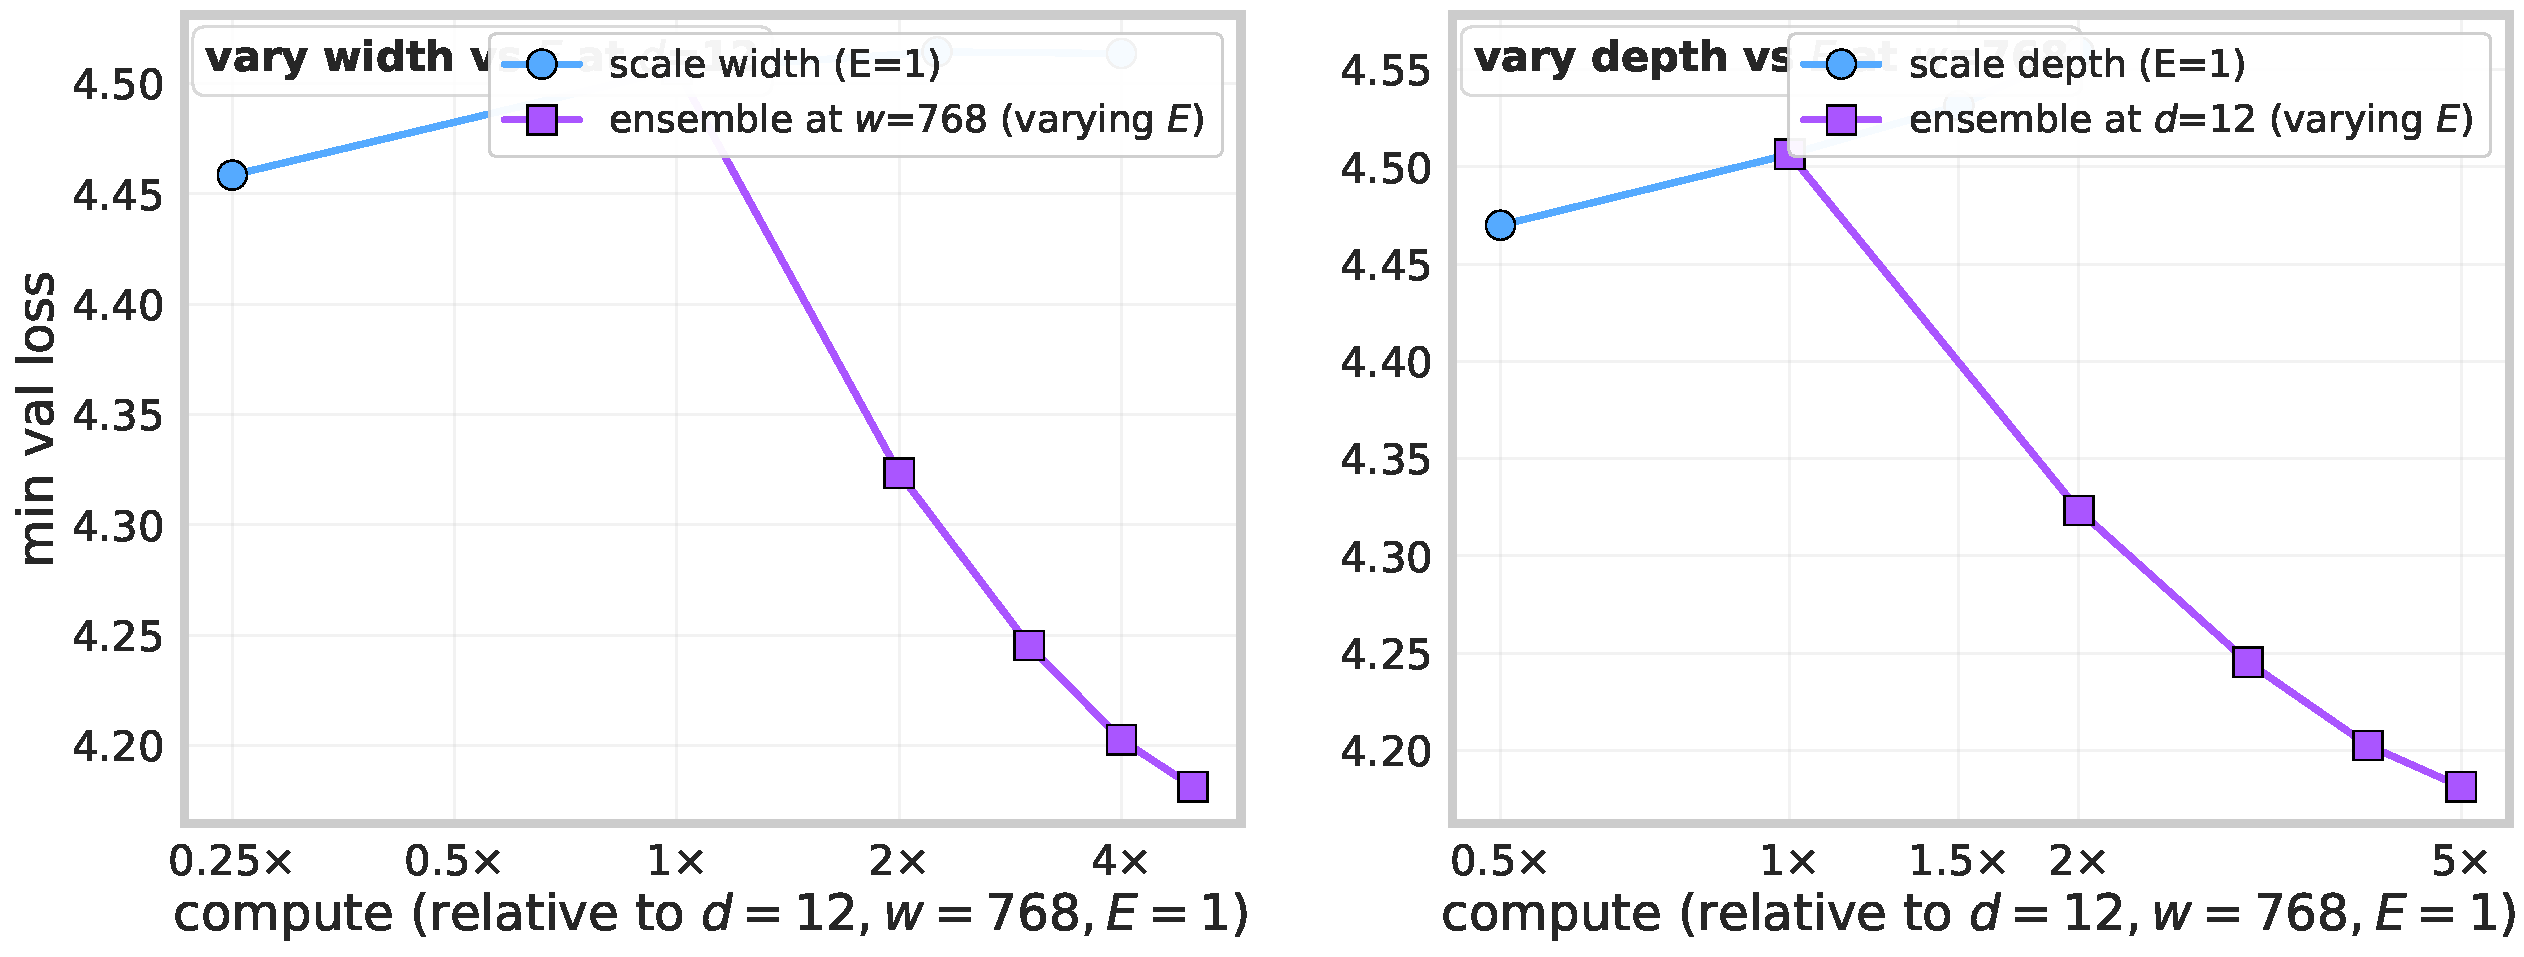
\includegraphics[width=0.99\linewidth]{experiments/figures/03_compute_matched/expt_fig3bc.pdf}
\caption{Compute-matched comparison: ensembling base-size models (purple squares) versus scaling a single model up (blue circles). Compute is normalized to the $d=12, w=768, E=1$ baseline. Left: width axis at $d=12$. Right: depth axis at $w=768$.}
\label{fig:compute_matched}
\end{figure}

\paragraph{Notes on Figure~\ref{fig:compute_matched}.}
Compute is taken to be proportional to the non-embedding parameter count $16 L N^2$ (for ensembles, multiplied by $E$).
For a single $d{=}12, w{=}768$ model the relative compute is $1\times$; doubling width to $w{=}1536$ gives $4\times$ ($N^2$); ensembling $E=4$ at the base gives $4\times$ as well.
The plotted $y$ value is the minimum validation loss attained over the 25-epoch training run, averaged across the 5 individuals (single-model points) or read from the ensemble replay (ensemble points).
Both panels use init plus shuffle.

% --- 3b/c body ---

The non-monotonicity of $L(t)$ in Figure~\ref{fig:overfit_u_curve} and the power-law $E$-dependence in Figure~\ref{fig:ensemble_scaling} together imply that ensembling at the base size and scaling up a single model are both ways to spend extra compute past the overfit-onset epoch.
Figure~\ref{fig:compute_matched} compares them directly at matched compute.
At $d=12$, scaling the single model from $w=768$ to $w=1536$ ($4\times$ compute via parameters) reduces minimum val loss only marginally, from $4.46$ to $4.50$ (it actually gets \emph{worse} in this data-limited regime, where the wider model overfits harder).
Ensembling at the base width buys $4\times$ compute via members and reduces the minimum val loss from $4.46$ at $E{=}1$ to $4.18$ at $E{=}4$, a $0.28$-nat improvement that the width-scaling channel does not deliver at any compute we tested.
The depth axis (right panel) shows the same qualitative result: increasing depth from $L=6$ to $L=24$ at $w=768$ does not lower the floor, and ensembling at $L=12$ dominates at every matched compute point.
This is the central operational claim of the paper: under data limits, additional FLOPs are best spent on members, not on parameters.


% --- 3d: heatmap ---

\begin{figure}[t]
\centering
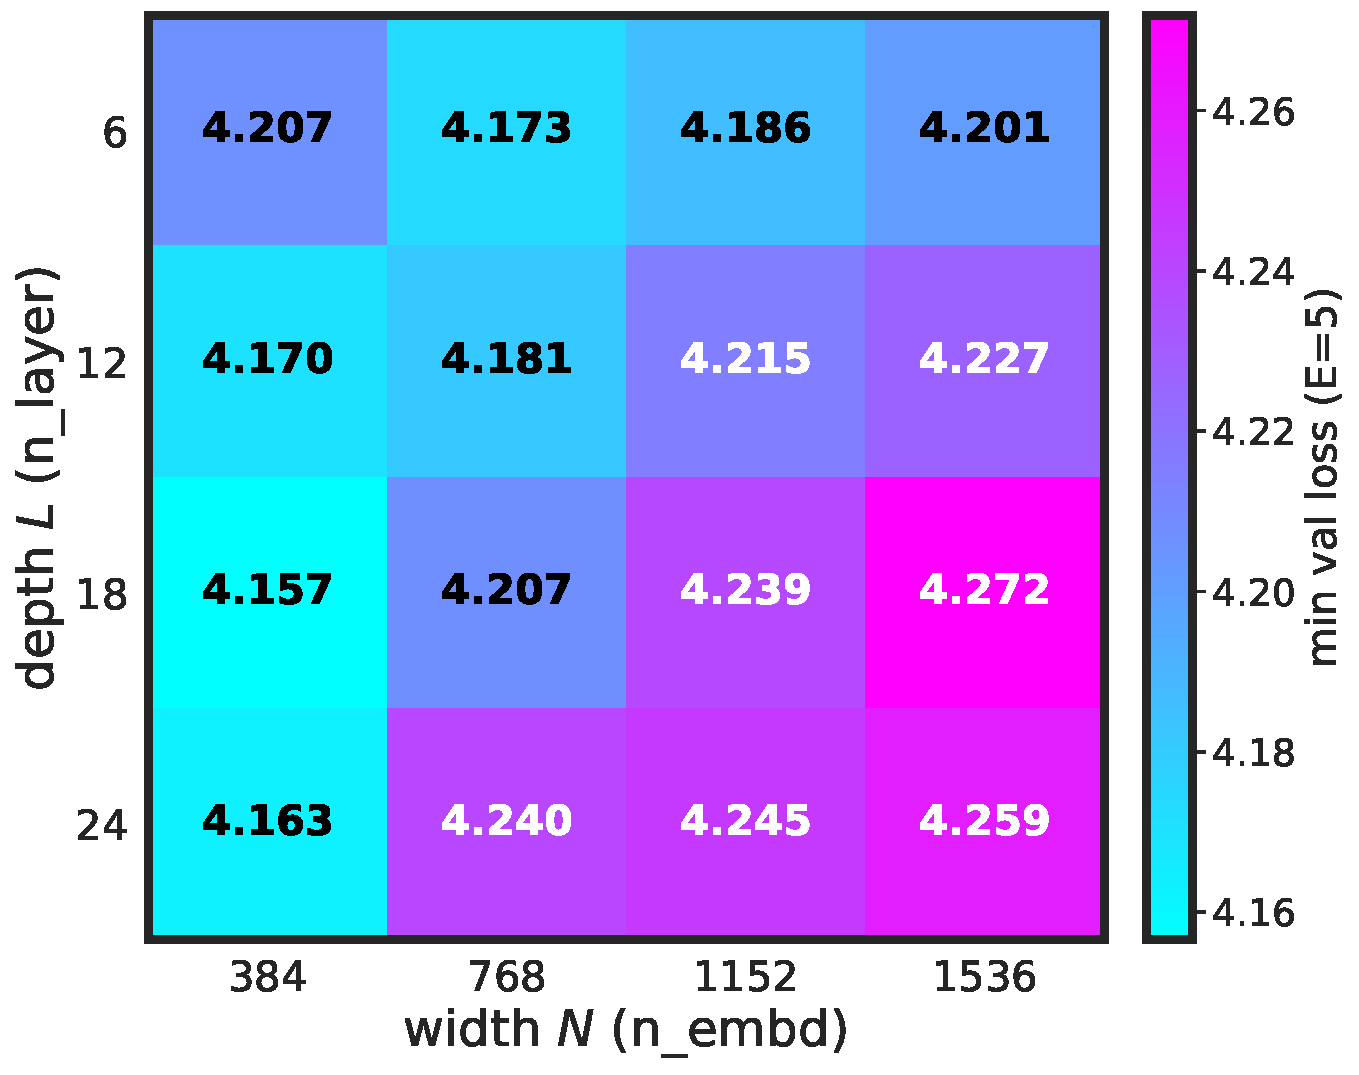
\includegraphics[width=0.55\linewidth]{experiments/figures/03_compute_matched/expt_fig3d_heatmap.pdf}
\caption{Minimum ensemble validation loss at $E=5$ across the $4 \times 4$ depth $\times$ width grid. Smaller width and moderate depth dominate.}
\label{fig:heatmap}
\end{figure}

\paragraph{Notes on Figure~\ref{fig:heatmap}.}
Each cell shows the minimum value of the $E=5$ ensemble val curve (init plus shuffle) over the 25-epoch run.
The optimal cell is $L=18, N=384$ at val $4.157$; the worst is $L=18, N=1536$ at val $4.272$, a spread of only $0.115$ nats across a $24\times$ range in non-embedding parameters.
Width hurts more than depth helps: the left column ($N=384$) dominates the right ($N=1536$) at every depth.


% --- 3e: scaling-law fit ---

\begin{figure}[t]
\centering
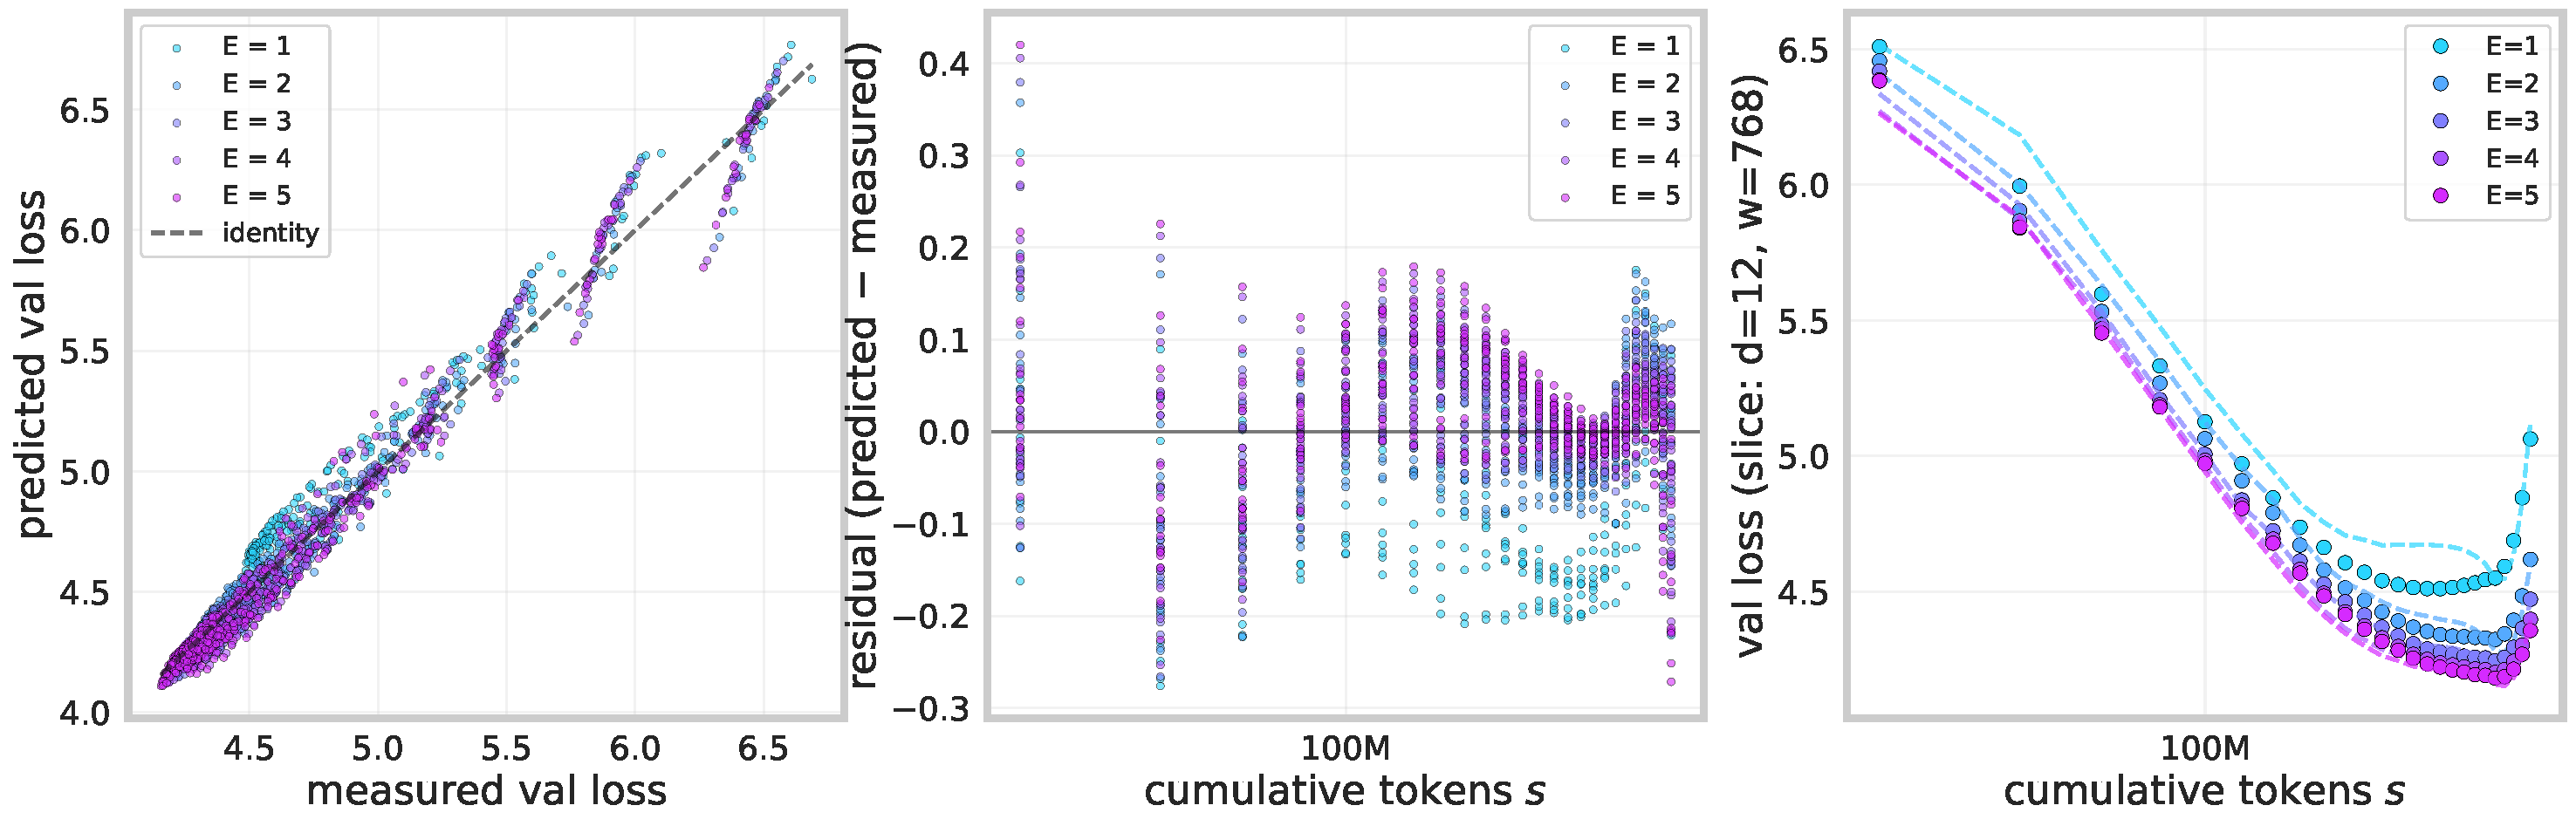
\includegraphics[width=0.99\linewidth]{experiments/figures/03_compute_matched/expt_fig3e_scaling_law.pdf}
\caption{Joint fit of the general scaling law to the entire $4 \times 4$ grid + ensembles. Left: predicted vs measured val loss (1825 points, identity line dashed). Middle: residuals vs cumulative tokens $s$, colored by $E$. Right: a representative slice ($d=12, w=768$); markers are observations, dashed lines are the joint-fit prediction.}
\label{fig:scaling_law}
\end{figure}

\paragraph{Notes on Figure~\ref{fig:scaling_law}.}
We fit the general form
$$\mathcal{L}(s, N, L, E) \;=\; c_t\,(s/s_0)^{-r_t} + c_p\,(N_r^2 L_r)^{-r_{\text{param}}} + c_v\,E^{-d_E}\,N_r^{d_N}\,L_r^{d_L}\,(s/s_0)^{d_t} + \mathcal{L}_0$$
with reference scales $s_0 = 300$M tokens, $N_0 = 768$, $L_0 = 12$ (so the reduced variables $s_r = s/s_0$, $N_r = N/N_0$, $L_r = L/L_0$ are $\mathcal{O}(1)$ at the base cell at the typical overfit-onset).
The data-limited $P^{-r_P}$ term is absorbed into $\mathcal{L}_0$ since $P$ (the unique-data fraction) is held fixed at $df=0.2$ across all 16 cells.
Joint nonlinear least-squares fit over 1825 measurements (16 cells $\times$ 5 ensemble sizes $\times \approx 25$ snapshots) and 10 free parameters.
The fit reaches per-observation residual $\hat\sigma = 0.083$ nats, well below the data range of $\approx 2.5$ nats; predicted vs measured (left panel) hugs the identity line.
Several parameters hit physical bounds, however, indicating that the joint identifiability with our 25-epoch data is limited: $\mathcal{L}_0 = 0$ (lower bound) and $d_t = 3.8$ near its upper bound suggest the bias-dynamics term and variance-buildup term jointly absorb the role of the Bayes-error floor.
The fit's central exponent $d_E = 0.56 \pm 0.01$ disagrees with Figure~\ref{fig:ensemble_scaling}'s $b = 1.15 \pm 0.03$ for the init plus shuffle strategy at base cell, which we attribute to the broader model averaging across cells with very different effective ensemble correlations.
A more pinned-down identification would require either longer training so that the variance-buildup term can be cleanly separated from the bias-dynamics term, or fixing $d_E$ from the per-cell measurement of Figure~\ref{fig:ensemble_scaling} as a prior in the joint fit.

% --- body ---

The general scaling law in Eq.~(1) of the introduction gathers all four contributions to the loss into a single closed form: bias dynamics ($s^{-r_t}$), parameters ($(N^2 L)^{-r_{\text{param}}}$), data-limited Bayes error ($P^{-r_P}$), and the variance-buildup term that simultaneously decreases in $E$ (the $E^{-\delta_E}$ factor) and increases in $s$, $N$, and $L$ (the $(s/T)^{\delta_t} N^{\delta_N} L^{\delta_L}$ factors).
Figure~\ref{fig:scaling_law} shows that this five-term form fits our $4 \times 4$ grid plus ensemble data with sub-tenth-nat residuals across the entire 1825-point set.
Two complications keep us from fully validating the theory's $\delta_E = 1$ conjecture from this fit alone.
First, with only 25 epochs at $df=0.2$, most of our cells barely complete one overfit cycle, so the variance-buildup term and the bias-dynamics term are poorly separated in $s$.
Second, the joint optimum places several parameters at the physical bounds we imposed, indicating that the data leaves a degenerate ridge in parameter space.
The cleaner identification comes from Figure~\ref{fig:ensemble_scaling}, which is a one-cell, time-resolved snapshot fit: there $\delta_E$ is well-identified per strategy and per snapshot $T$, and the answer is that init plus shuffle gives $b \approx 1.15$ while init only gives $b \approx 0.75$, bracketing the theoretical conjecture $\delta_E = 1$.
Reading Figures~\ref{fig:ensemble_scaling} and~\ref{fig:scaling_law} together, the picture is that the variance-buildup term is the operationally important one: it explains why ensembling beats single-model scaling at matched compute, and its $E^{-\delta_E}$ factor with $\delta_E$ close to (or above) $1$ guarantees that the gain from each additional member is at least as large as a $1/E$ noise-averaging would predict.
